%!TEX root = ../../thesis.tex

\section{Why should we correct classifiers' predictions}
\label{chapter:limitiations:simplevsmatching}

We compare the performance of Equation~\ref{eq:matchingfilter} and Equation~\ref{eq:matchingfiltercrossvalidation} defined in chapter~\ref{chapter:lfui}. The main difference these two equation is that the second (Equation~\ref{eq:matchingfiltercrossvalidation}) is adding an other layer of verification, by estimating the intrinsic quality of the classifier used to classify the new observation. In others words, we temperate the prediction of the classifier given our knowledge about its quality, which we measure by computing the confusion matrix via a cross-validation procedure.

\subsection{Artificial data}

We consider the same setting as for the experiments described in chapter~\ref{chapter:bci:EEGsignals} and used our 2 dimensional dataset of different quality as presented in chapter~\ref{chapter:planning:artificialsignals}. We ran 500 simulations for each method. We consider only the active planning method used in chapter~\ref{chapter:planning}.

\paragraph{Time to first task} Figure~\ref{fig:timefirst_simplevsmatching} compares the number of iterations needed to identify the first time with confidence between our two methods. We call the method using equation Equation~\ref{eq:matchingfilter} ``simple matching'' and we call ``matching'' the method using Equation~\ref{eq:matchingfiltercrossvalidation} which correct the classifier prediction. There is strong differences between our method especially for low quality dataset. For extremely overlapping data (50/60\% accuracy), the ``matching'' method is never confident about a task while the ``simple matching'' method show huge variability and sometime outputs confidence after very few time steps. 

\begin{figure}[!htbp]
\centering
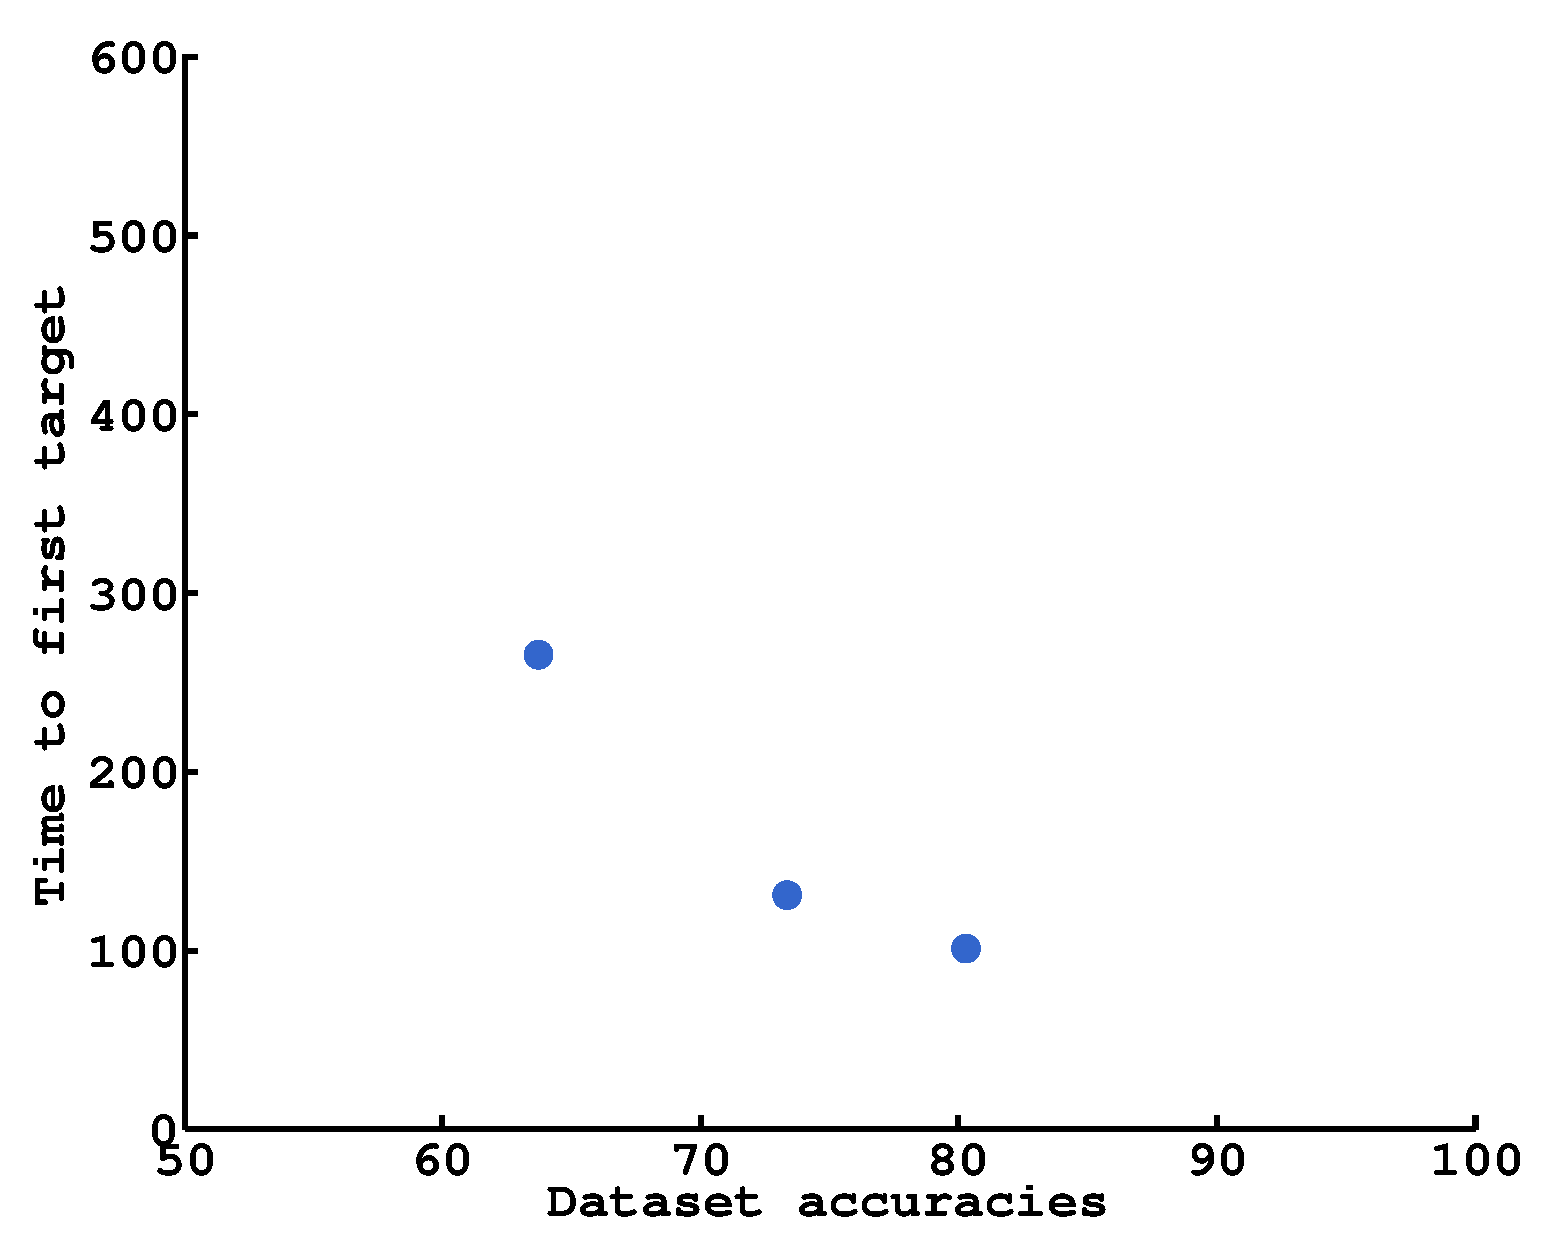
\includegraphics[width=\plotsize\columnwidth]{\imgpath/simplevsmatching/timefirst.eps}
\caption{Number of steps to complete first task with high quality 2D dataset. Comparison between Equation~\ref{eq:matchingfilter} (simple matching) and Equation~\ref{eq:matchingfiltercrossvalidation} (matching), where the latter correct the prediction of the classifier given the estimation of its confusion matrix.}
\label{fig:timefirst_simplevsmatching}
\end{figure} 

This over confidence of the ``simple matching'' method reflects in the number of first task that were erroneously identified. As shown in Table~\ref{tab:errorTaskRatiosimplevsmatching}, the lower the quality of the data, the higher the percentage of erroneously identified first task. For extremely overlapping data (50/60\% accuracy), this percentage go up to 20 percent. While the ``matching'' method may seems too conservative, it is particularly important to not make mistakes when estimating the first task. Indeed once a first task is identified, its associated labels are taken as ground truth, and a false estimation will falsify the signal-label pairs for the remaining of the interaction.

\begin{table}[!htbp]
\centering
\rowcolors{2}{gray!25}{white}
\begin{tabular}{c c c c}
    Dataset Accuracies & Simple Matching &  Matching \\ \hline
    50-60 & 0.21 & 0 \\ 
    60-70 & 0.16 & 0 \\
    70-80 & 0.03 & 0 \\
    80-90 & 0.02 & 0 \\
    90-100 & 0.01 & 0 \\
\end{tabular}
\caption{Percentage of time the first task estimated was erroneous using a high quality 2D dataset. Comparison between Equation~\ref{eq:matchingfilter} (simple matching) and Equation~\ref{eq:matchingfiltercrossvalidation} (matching), where the latter correct the prediction of the classifier given the estimation of its confusion matrix. Only the ``matching'' method that temperates the prediction of the classifier do not make mistake when estimating the first task.}
\label{tab:errorTaskRatiosimplevsmatching}
\end{table}

\paragraph{Number of tasks achieved in 500 steps}

We compare the number of task correctly (Figure~\ref{fig:nCorrect_simplevsmatching}) and incorrectly (Figure~\ref{fig:nWrongEEG_simplevsmatching}) reached in 500 steps between our two methods. While the ``simple matching'' allow to reach more target correctly is also makes mistakes for low quality datasets. The ``matching'' method is more conservative and do not make mistake for all classifier qualities, at the cost of reaching less targets.

\begin{figure}[!htbp]
\centering
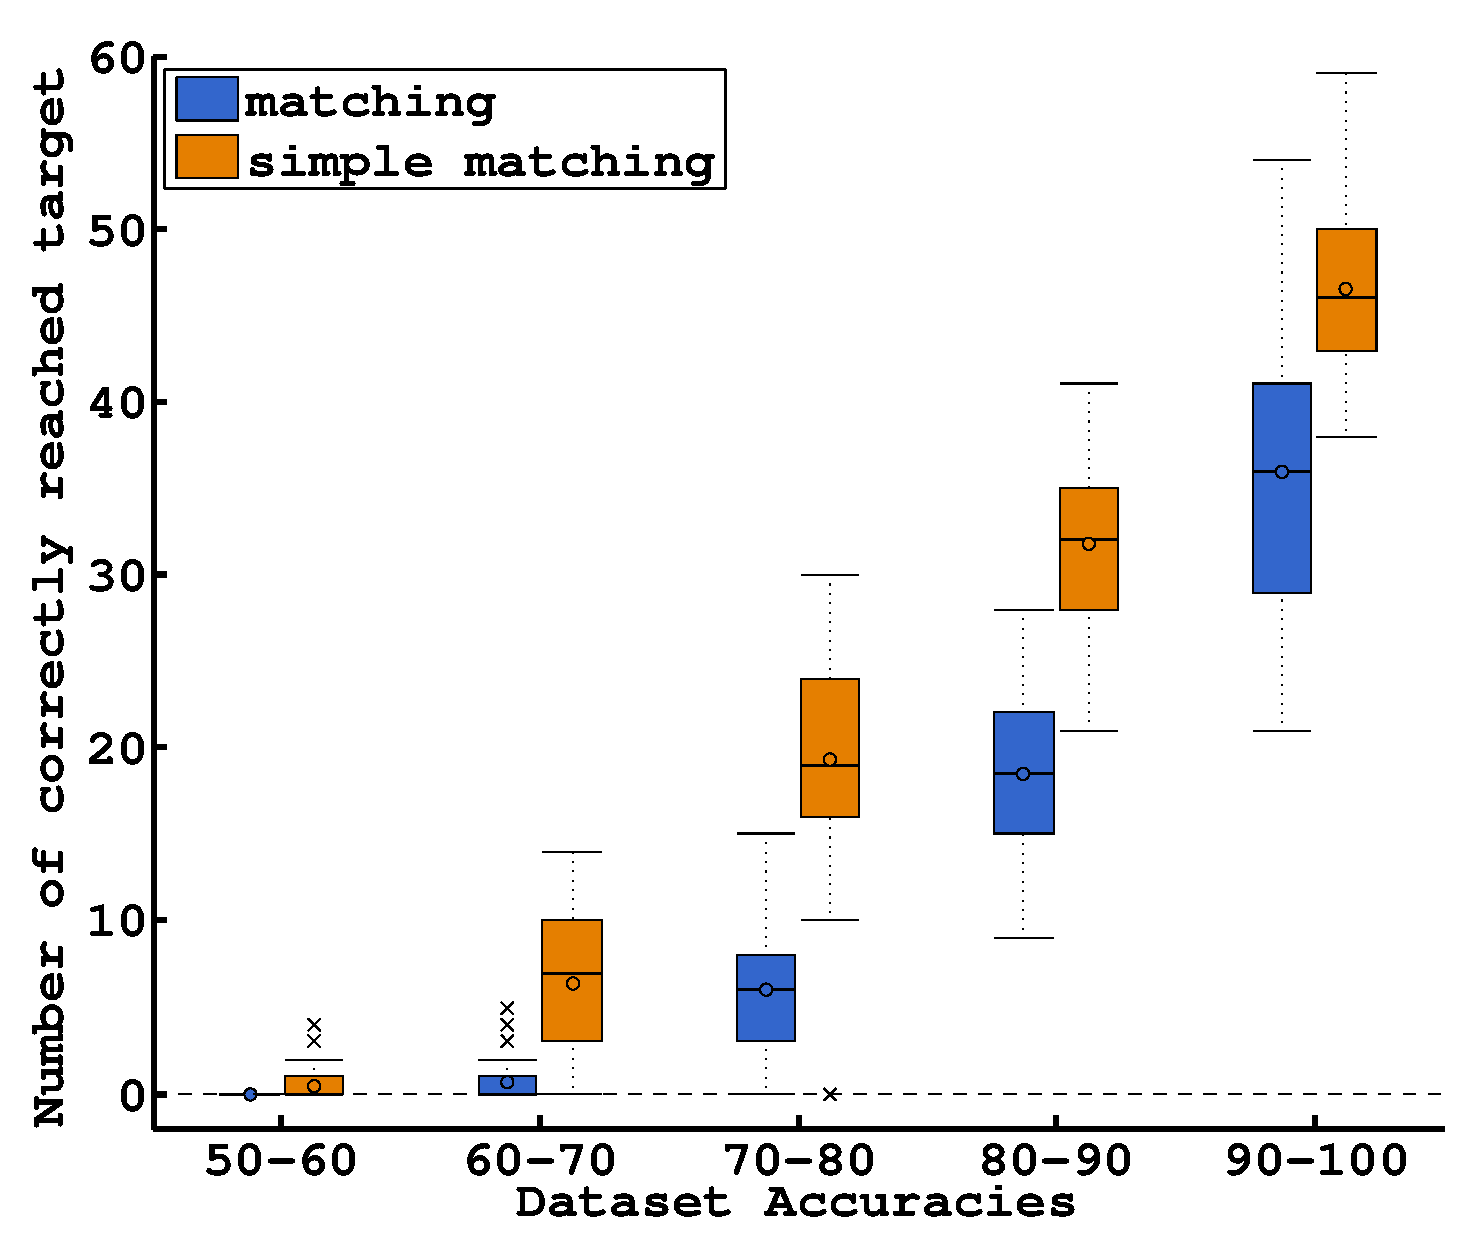
\includegraphics[width=\plotsize\columnwidth]{\imgpath/simplevsmatching/correct.eps}
\caption{Number of task correctly achieved in 500 steps with 2 dimensional artificial data. Comparison between Equation~\ref{eq:matchingfilter} (simple matching) and Equation~\ref{eq:matchingfiltercrossvalidation} (matching), where the latter correct the prediction of the classifier given the estimation of its confusion matrix. The ``simple matching'' method allow to reach more task correctly in 500 steps for all dataset quality.
}
\label{fig:nCorrect_simplevsmatching}
\end{figure} 

\begin{figure}[!htbp]
\centering
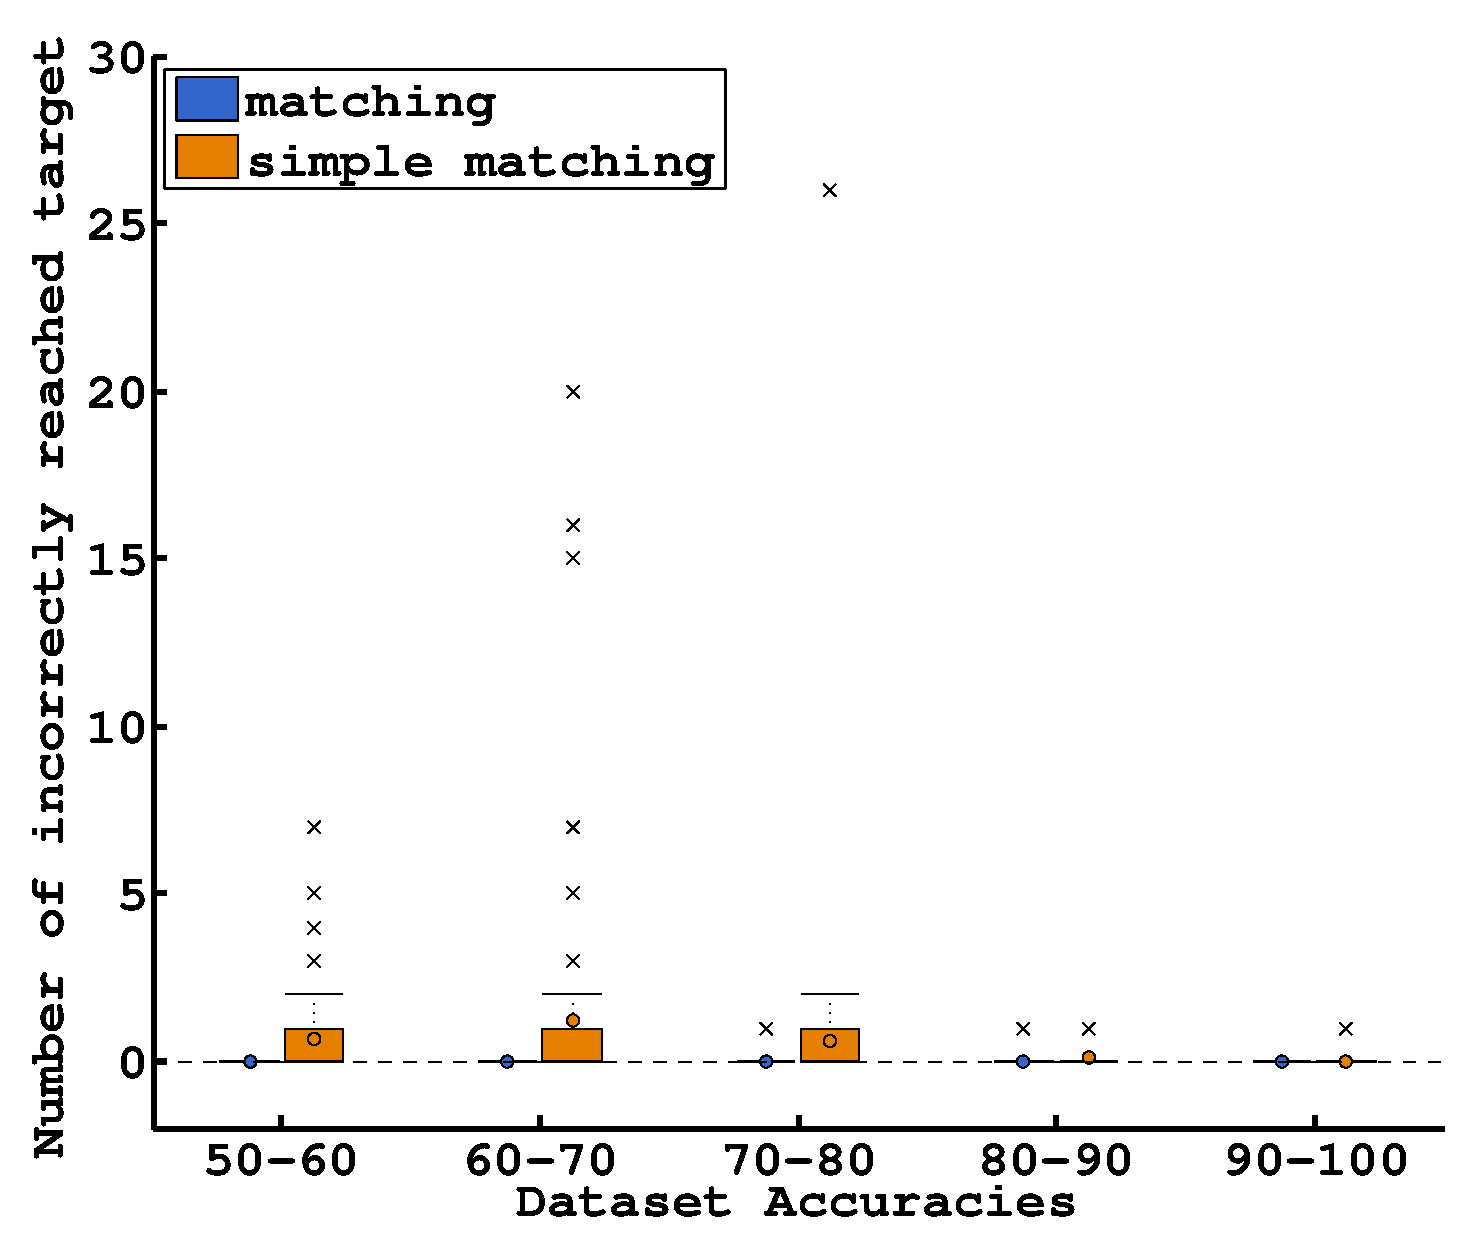
\includegraphics[width=\plotsize\columnwidth]{\imgpath/simplevsmatching/error.eps}
\caption{Number of task incorrectly achieved in 500 steps with 2 dimensional artificial data. Comparison between Equation~\ref{eq:matchingfilter} (simple matching) and Equation~\ref{eq:matchingfiltercrossvalidation} (matching), where the latter correct the prediction of the classifier given the estimation of its confusion matrix. The ``simple matching'' method start making errors for dataset with accuracies lower than 80 percent classification rate. However, the ``matching'' method is more conservative and do not make mistakes.}
\label{fig:nWrongEEG_simplevsmatching}
\end{figure} 

\transition

Those results considered only low dimensional dataset (2D), which were generated from Gaussian distribution which match perfectly with the assumption made by our classifier. The combination of those two factors makes it easy to find which classifier is the correct one. We now investigate how those properties are affected by more complex signals, such as the EEG datasets used in chapter~\ref{chapter:bci}, which are 34 dimensional with data distribution that do not necessarily follow the Gaussian assumption.

\subsection{EEG data}

We consider now the same setting as for the previous subsection but use our EEG datasets described in chapter~\ref{chapter:bci}. We ran 500 simulations for each method. We consider only the active planning method used in chapter~\ref{chapter:planning}.

\paragraph{Time to first task} Figure~\ref{fig:timefirst_simplevsmatchingEEG} compares the number of iterations needed to identify the first time with confidence between our two methods. There is strong differences between our method especially for low quality dataset. The ``simple matching'' method performances are not correlated with the classifier qualities, which reflect the overconfidence of this method.

\begin{figure}[!htbp]
\centering
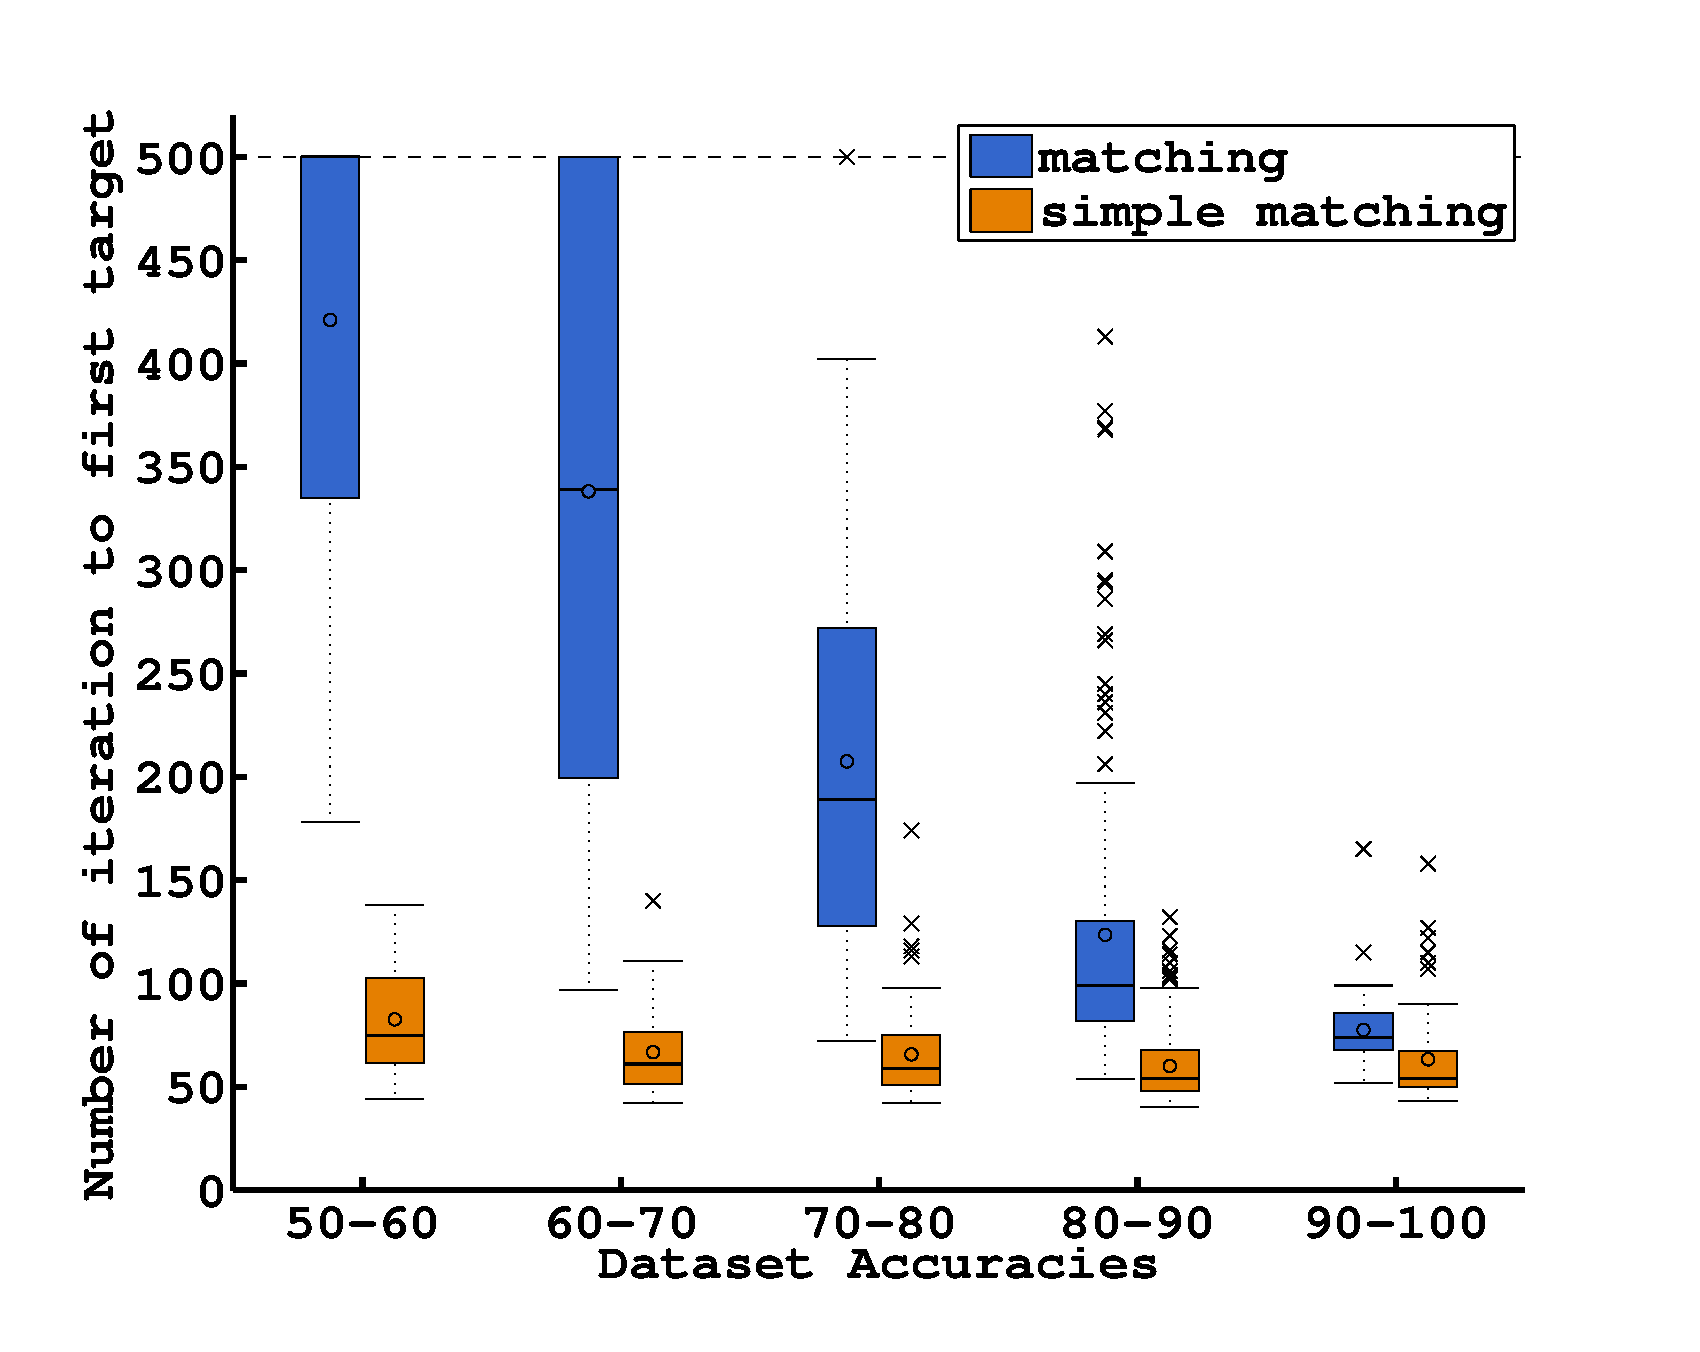
\includegraphics[width=\plotsize\columnwidth]{\imgpath/simplevsmatching/timefirstEEG.eps}
\caption{Number of steps to complete first task with our pre-recorded EEG data. Comparison between Equation~\ref{eq:matchingfilter} (simple matching) and Equation~\ref{eq:matchingfiltercrossvalidation} (matching), where the latter correct the prediction of the classifier given the estimation of its confusion matrix. The ``simple matching'' method performances are not correlated with the classifier qualities, which is not a good property. Indeed as reported in Table~\ref{tab:errorTaskRatiosimplevsmatchingEEG} the ``simple matching'' method is estimating more than 50 percent fo the time the first task erroneously.}
\label{fig:timefirst_simplevsmatchingEEG}
\end{figure} 

This over confidence of the ``simple matching'' method reflects in the number of first task that were erroneously identified. As shown in Table~\ref{tab:errorTaskRatiosimplevsmatchingEEG}, the lower the quality of the data, the higher the percentage of erroneously identified first task. In all cases, this percentage was above 50 percent which make the use of the ``simple matching'' method impossible in practical experiment. On the contrary, the ``matching'' method do not make any mistake when estimating the first task.

\begin{table}[!htbp]
\centering
\rowcolors{2}{gray!25}{white}
\begin{tabular}{c c c c}
    Dataset Accuracies & Simple Matching &  Matching \\ \hline
    50-60 & 0.81 & 0 \\ 
    60-70 & 0.80 & 0 \\
    70-80 & 0.66 & 0 \\
    80-90 & 0.53 & 0 \\
    90-100 & 0.60 & 0 \\
\end{tabular}
\caption{Percentage of time the first task estimated was erroneous using our pre-recorded EEG data. Comparison between Equation~\ref{eq:matchingfilter} (simple matching) and Equation~\ref{eq:matchingfiltercrossvalidation} (matching), where the latter correct the prediction of the classifier given the estimation of its confusion matrix. Only the ``matching'' method that temperates the prediction of the classifier do not make mistake when estimating the first task.}
\label{tab:errorTaskRatiosimplevsmatchingEEG}
\end{table}

\paragraph{Number of tasks achieved in 500 steps}

We compare the number of task correctly (Figure~\ref{fig:nCorrect_simplevsmatchingEEG}) and incorrectly (Figure~\ref{fig:nWrongEEG_simplevsmatchingEEG}) reached in 500 steps between our two methods. While the two methods allow to reach a similar number of targets correctly. The ``simple matching'' method also makes a huge amount of mistakes for all datasets. The ``matching'' method makes very few mistakes for all classifier qualities.

\begin{figure}[!htbp]
\centering
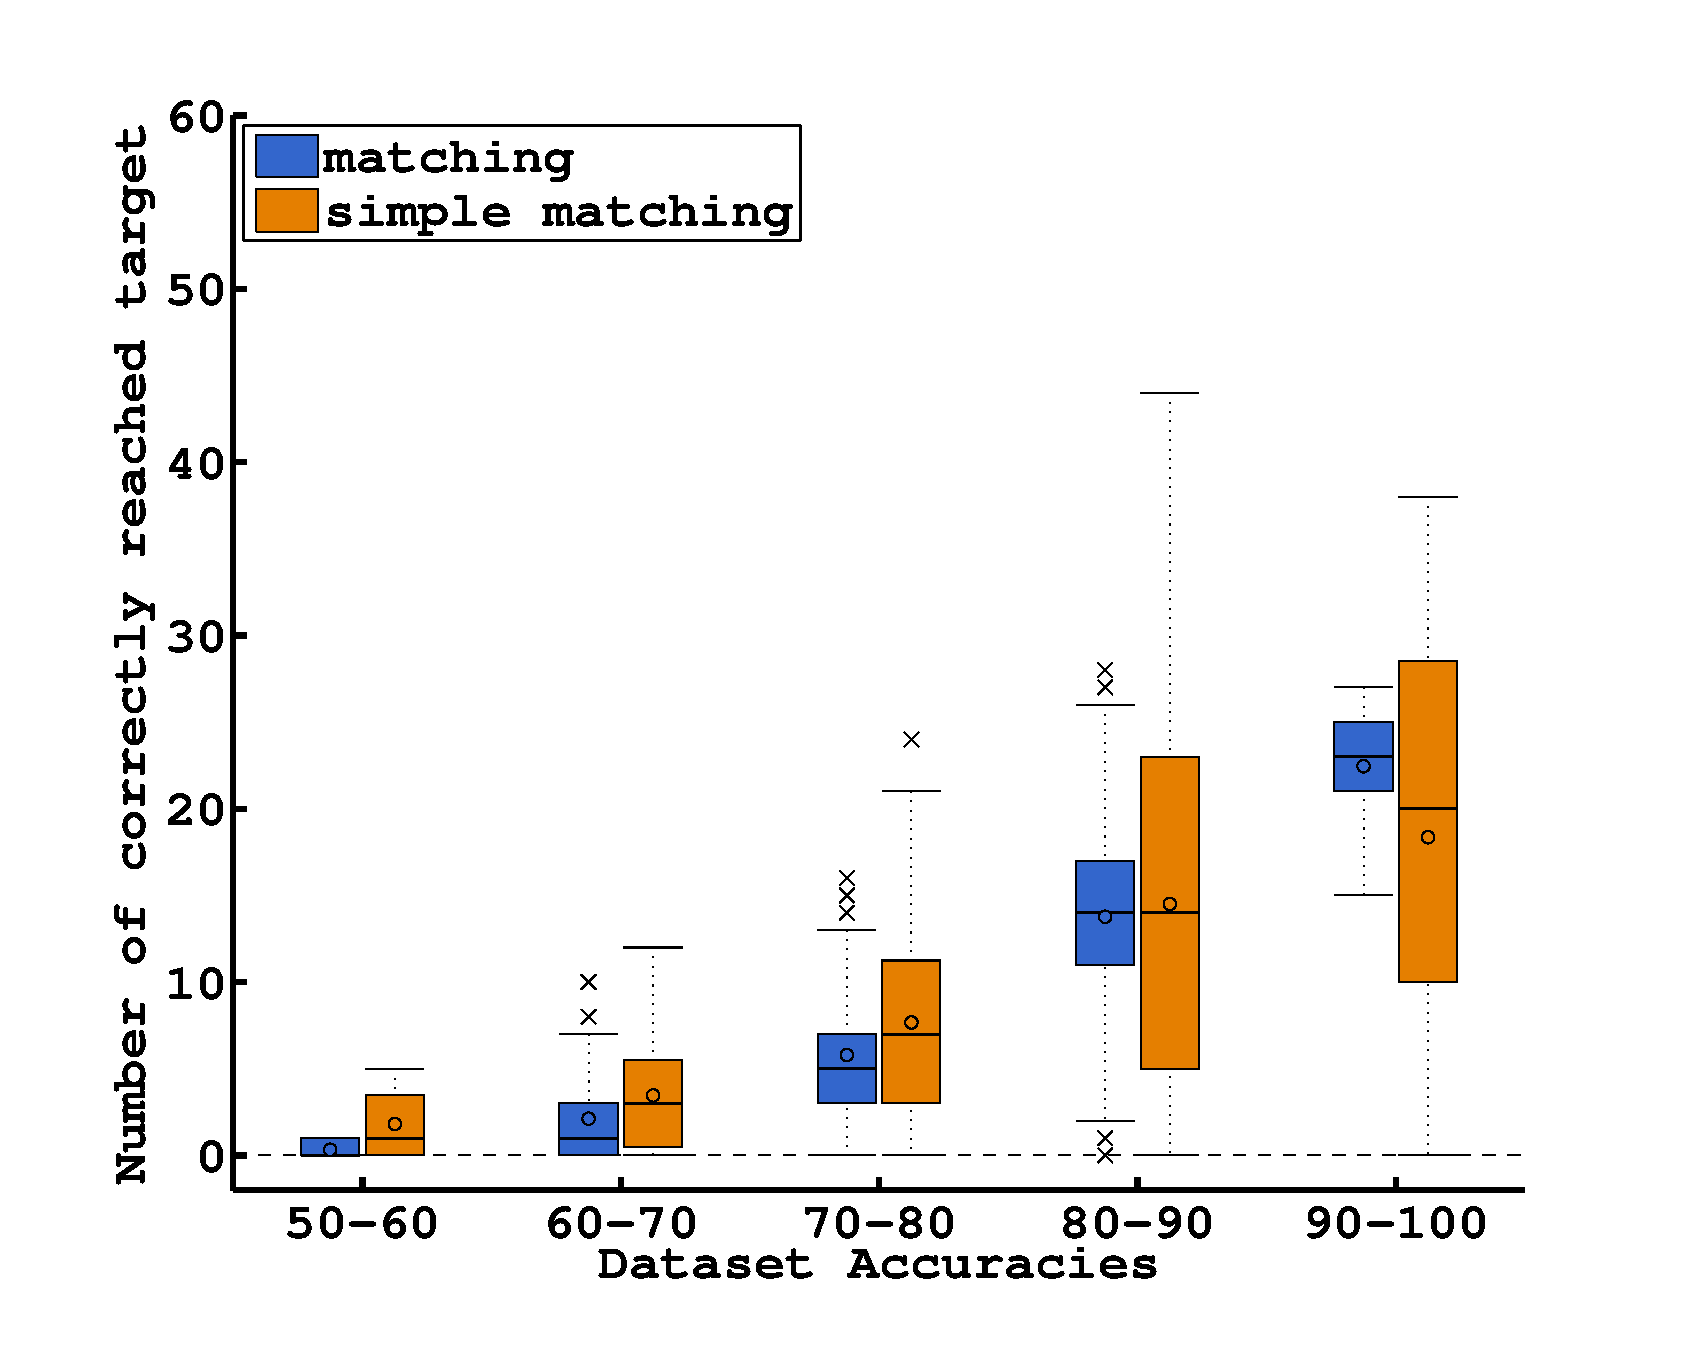
\includegraphics[width=\plotsize\columnwidth]{\imgpath/simplevsmatching/correctEEG.eps}
\caption{Number of task correctly achieved in 500 steps with our pre-recorded EEG data. Comparison between Equation~\ref{eq:matchingfilter} (simple matching) and Equation~\ref{eq:matchingfiltercrossvalidation} (matching), where the latter correct the prediction of the classifier given the estimation of its confusion matrix. Both method reach a similar number of targets correctly when using an EEG datset. The ``simple matching''  method shows more variability.}
\label{fig:nCorrect_simplevsmatchingEEG}
\end{figure} 

\begin{figure}[!htbp]
\centering
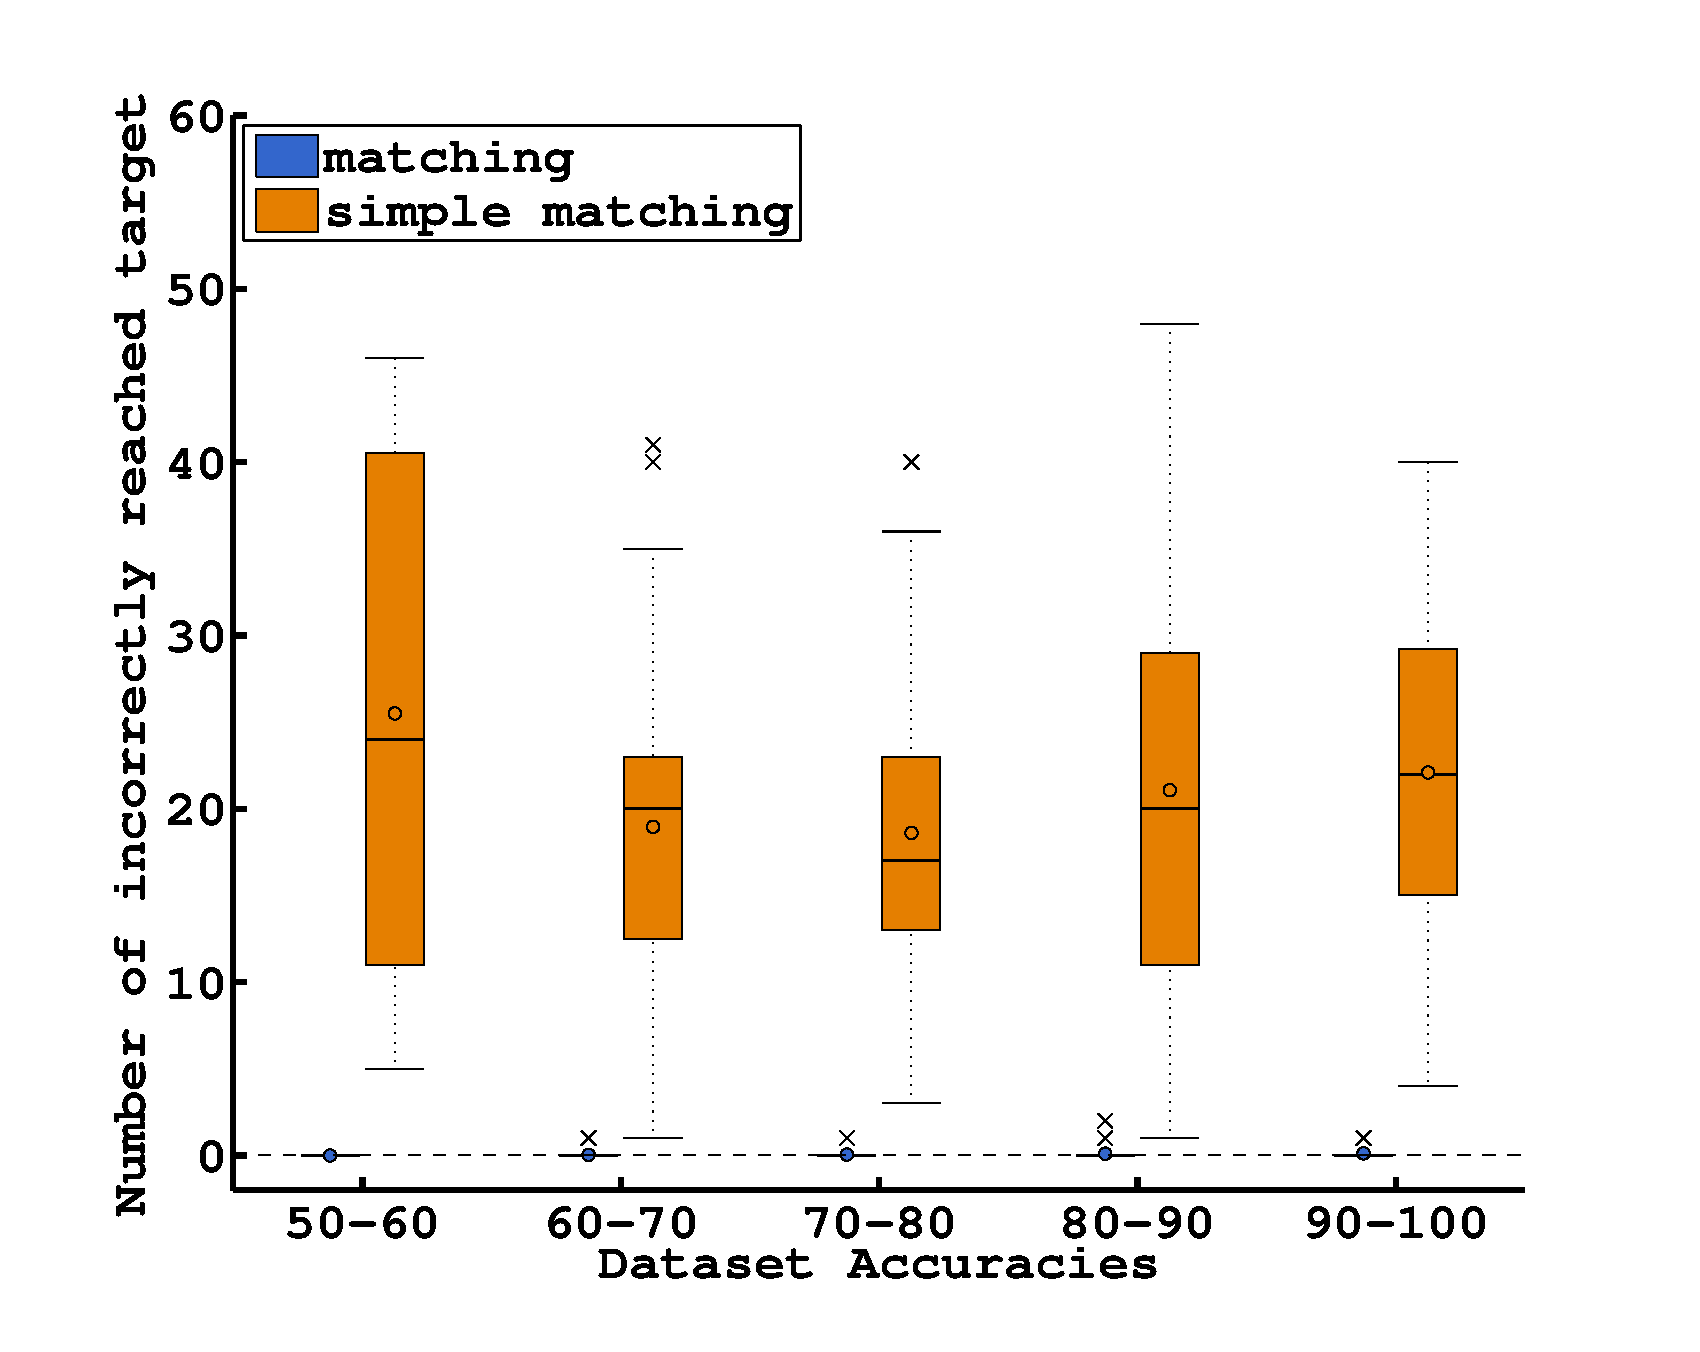
\includegraphics[width=\plotsize\columnwidth]{\imgpath/simplevsmatching/errorEEG.eps}
\caption{Number of task incorrectly achieved in 500 steps with our pre-recorded EEG data. Comparison between Equation~\ref{eq:matchingfilter} (simple matching) and Equation~\ref{eq:matchingfiltercrossvalidation} (matching), where the latter correct the prediction of the classifier given the estimation of its confusion matrix. The ``simple matching'' is not reliable for EEG data.}
\label{fig:nWrongEEG_simplevsmatchingEEG}
\end{figure} 

\subsection{Discussion}

Our results confirms that using the uncertainty about the prediction of our classifier makes our algorithm more robust. However if we knew the data will be of good enough quality and respect the assumtion made by our classifiers, we could afford not correcting the classifiers' outputs (as with the speech dataset used in chapter~\ref{chapter:lfui}), but as soon as we have to deal with a variety of signals quality and properties (like for BCI in chapter~\ref{chapter:bci}) it is better to include a measure of classification quality on our likelihood update rule.